\documentclass{standalone}
\usepackage{tikz}
\usetikzlibrary{patterns, positioning}

\begin{document}
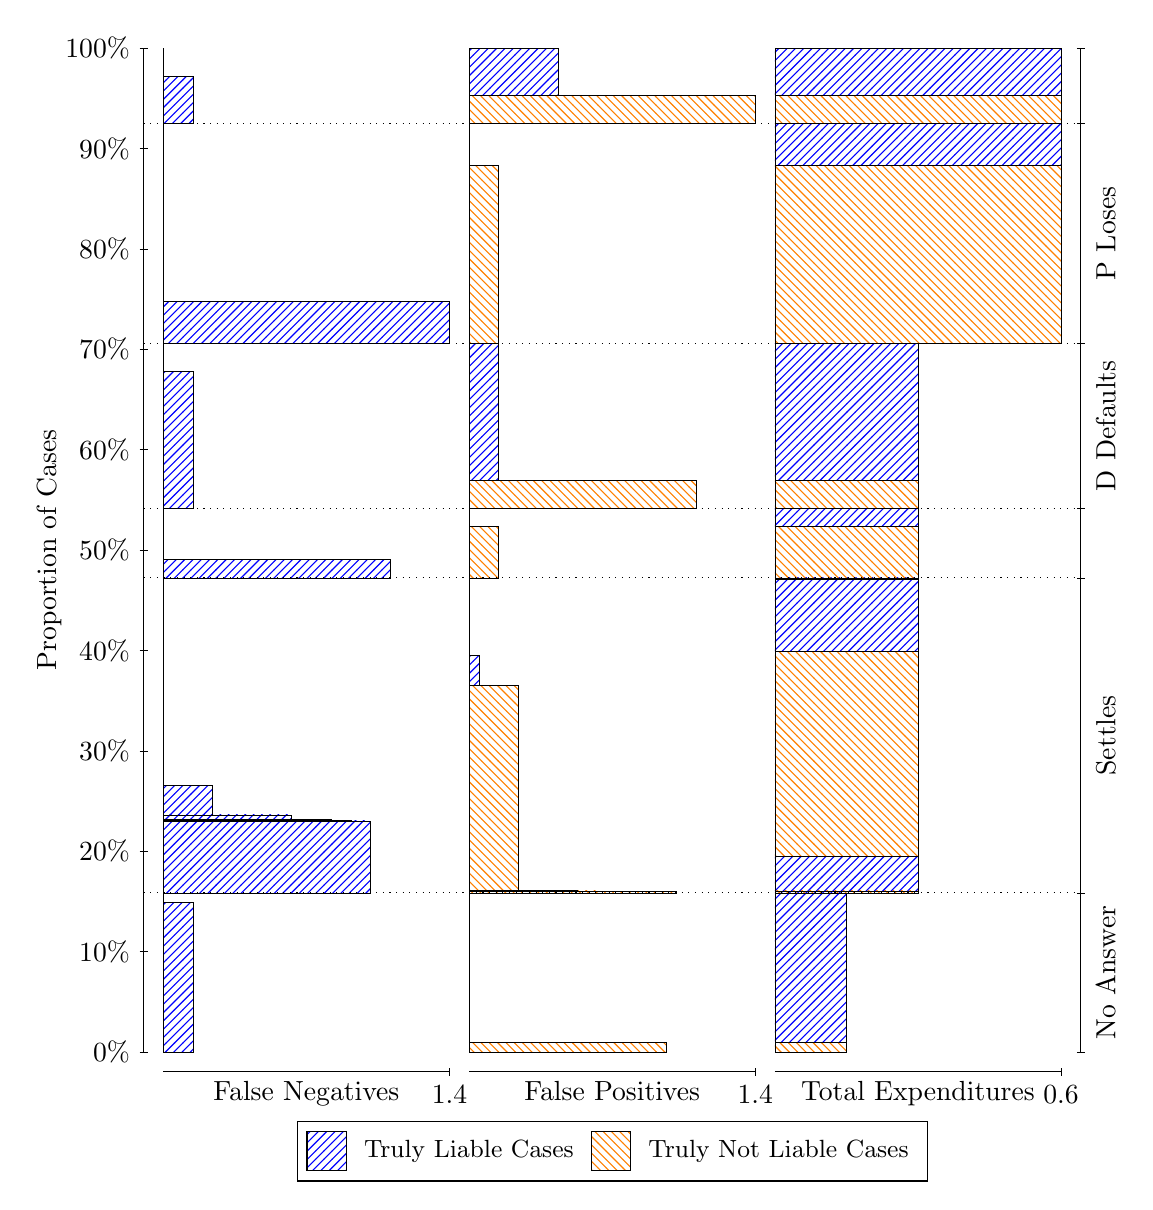
\begin{tikzpicture}
\draw[black, very thin] (1.5,1.75) -- (1.5,14.5);
\node[rotate=90, anchor=center] at (0.3, 8.125) {Proportion of Cases};
\draw[black, very thin] (1.45,1.75) -- (1.55,1.75);
\node[anchor=east] at (1.45, 1.75) {0\%};
\draw[black, very thin] (1.45,3.025) -- (1.55,3.025);
\node[anchor=east] at (1.45, 3.025) {10\%};
\draw[black, very thin] (1.45,4.3) -- (1.55,4.3);
\node[anchor=east] at (1.45, 4.3) {20\%};
\draw[black, very thin] (1.45,5.575) -- (1.55,5.575);
\node[anchor=east] at (1.45, 5.575) {30\%};
\draw[black, very thin] (1.45,6.85) -- (1.55,6.85);
\node[anchor=east] at (1.45, 6.85) {40\%};
\draw[black, very thin] (1.45,8.125) -- (1.55,8.125);
\node[anchor=east] at (1.45, 8.125) {50\%};
\draw[black, very thin] (1.45,9.4) -- (1.55,9.4);
\node[anchor=east] at (1.45, 9.4) {60\%};
\draw[black, very thin] (1.45,10.675) -- (1.55,10.675);
\node[anchor=east] at (1.45, 10.675) {70\%};
\draw[black, very thin] (1.45,11.95) -- (1.55,11.95);
\node[anchor=east] at (1.45, 11.95) {80\%};
\draw[black, very thin] (1.45,13.225) -- (1.55,13.225);
\node[anchor=east] at (1.45, 13.225) {90\%};
\draw[black, very thin] (1.45,14.5) -- (1.55,14.5);
\node[anchor=east] at (1.45, 14.5) {100\%};

\draw[black, very thin] (13.4,1.75) -- (13.4,14.5);
\draw[black, very thin] (13.35,1.75) -- (13.45,1.75);
\node[anchor=west] at (13.35, 1.75) {};
\draw[black, very thin] (13.35,3.77) -- (13.45,3.77);
\node[anchor=west] at (13.35, 3.77) {};
\draw[black, very thin] (13.35,7.7716) -- (13.45,7.7716);
\node[anchor=west] at (13.35, 7.7716) {};
\draw[black, very thin] (13.35,8.6521) -- (13.45,8.6521);
\node[anchor=west] at (13.35, 8.6521) {};
\draw[black, very thin] (13.35,10.753) -- (13.45,10.753);
\node[anchor=west] at (13.35, 10.753) {};
\draw[black, very thin] (13.35,13.54) -- (13.45,13.54);
\node[anchor=west] at (13.35, 13.54) {};
\draw[black, very thin] (13.35,14.5) -- (13.45,14.5);
\node[anchor=west] at (13.35, 14.5) {};

\draw[black, very thin, pattern color=blue, pattern=north east lines] (1.75,1.75) rectangle (2.1259,3.6516);
\draw[black, very thin, pattern color=orange, pattern=north west lines] (1.75,3.6516) rectangle (1.75,3.77);
\draw[black, very thin, pattern color=blue, pattern=north east lines] (1.75,3.77) rectangle (4.381,4.6848);
\draw[black, very thin, pattern color=blue, pattern=north east lines] (1.75,4.6848) rectangle (4.1305,4.6919);
\draw[black, very thin, pattern color=blue, pattern=north east lines] (1.75,4.6919) rectangle (3.8799,4.699);
\draw[black, very thin, pattern color=blue, pattern=north east lines] (1.75,4.699) rectangle (3.6293,4.7061);
\draw[black, very thin, pattern color=blue, pattern=north east lines] (1.75,4.7061) rectangle (3.3787,4.7597);
\draw[black, very thin, pattern color=blue, pattern=north east lines] (1.75,4.7597) rectangle (2.3764,5.1396);
\draw[black, very thin, pattern color=orange, pattern=north west lines] (1.75,5.1396) rectangle (1.75,7.7716);
\draw[black, very thin, pattern color=blue, pattern=north east lines] (1.75,7.7716) rectangle (4.6316,8.003);
\draw[black, very thin, pattern color=orange, pattern=north west lines] (1.75,8.003) rectangle (1.75,8.6521);
\draw[black, very thin, pattern color=blue, pattern=north east lines] (1.75,8.6521) rectangle (2.1259,10.395);
\draw[black, very thin, pattern color=orange, pattern=north west lines] (1.75,10.395) rectangle (1.75,10.753);
\draw[black, very thin, pattern color=blue, pattern=north east lines] (1.75,10.753) rectangle (5.3833,11.279);
\draw[black, very thin, pattern color=orange, pattern=north west lines] (1.75,11.279) rectangle (1.75,13.54);
\draw[black, very thin, pattern color=blue, pattern=north east lines] (1.75,13.54) rectangle (2.1259,14.144);
\draw[black, very thin, pattern color=orange, pattern=north west lines] (1.75,14.144) rectangle (1.75,14.5);
\draw[black, very thin, pattern color=orange, pattern=north west lines] (5.6333,1.75) rectangle (8.1391,1.8684);
\draw[black, very thin, pattern color=blue, pattern=north east lines] (5.6333,1.8684) rectangle (5.6333,3.77);
\draw[black, very thin, pattern color=orange, pattern=north west lines] (5.6333,3.77) rectangle (8.2644,3.7931);
\draw[black, very thin, pattern color=orange, pattern=north west lines] (5.6333,3.7931) rectangle (7.2621,3.797);
\draw[black, very thin, pattern color=orange, pattern=north west lines] (5.6333,3.797) rectangle (7.0115,3.7976);
\draw[black, very thin, pattern color=orange, pattern=north west lines] (5.6333,3.7976) rectangle (6.7609,3.7981);
\draw[black, very thin, pattern color=orange, pattern=north west lines] (5.6333,3.7981) rectangle (6.5103,3.7986);
\draw[black, very thin, pattern color=orange, pattern=north west lines] (5.6333,3.7986) rectangle (6.2598,6.402);
\draw[black, very thin, pattern color=blue, pattern=north east lines] (5.6333,6.402) rectangle (5.7586,6.7819);
\draw[black, very thin, pattern color=blue, pattern=north east lines] (5.6333,6.7819) rectangle (5.6333,7.7716);
\draw[black, very thin, pattern color=orange, pattern=north west lines] (5.6333,7.7716) rectangle (6.0092,8.4207);
\draw[black, very thin, pattern color=blue, pattern=north east lines] (5.6333,8.4207) rectangle (5.6333,8.6521);
\draw[black, very thin, pattern color=orange, pattern=north west lines] (5.6333,8.6521) rectangle (8.5149,9.0101);
\draw[black, very thin, pattern color=blue, pattern=north east lines] (5.6333,9.0101) rectangle (6.0092,10.753);
\draw[black, very thin, pattern color=orange, pattern=north west lines] (5.6333,10.753) rectangle (6.0092,13.014);
\draw[black, very thin, pattern color=blue, pattern=north east lines] (5.6333,13.014) rectangle (5.6333,13.54);
\draw[black, very thin, pattern color=orange, pattern=north west lines] (5.6333,13.54) rectangle (9.2667,13.896);
\draw[black, very thin, pattern color=blue, pattern=north east lines] (5.6333,13.896) rectangle (6.7609,14.5);
\draw[black, very thin, pattern color=orange, pattern=north west lines] (9.5167,1.75) rectangle (10.425,1.8684);
\draw[black, very thin, pattern color=blue, pattern=north east lines] (9.5167,1.8684) rectangle (10.425,3.77);
\draw[black, very thin, pattern color=orange, pattern=north west lines] (9.5167,3.77) rectangle (11.333,3.797);
\draw[black, very thin, pattern color=blue, pattern=north east lines] (9.5167,3.797) rectangle (11.333,4.2305);
\draw[black, very thin, pattern color=orange, pattern=north west lines] (9.5167,4.2305) rectangle (11.333,6.8339);
\draw[black, very thin, pattern color=blue, pattern=north east lines] (9.5167,6.8339) rectangle (11.333,7.7487);
\draw[black, very thin, pattern color=orange, pattern=north west lines] (9.5167,7.7487) rectangle (11.333,7.7502);
\draw[black, very thin, pattern color=blue, pattern=north east lines] (9.5167,7.7502) rectangle (11.333,7.7716);
\draw[black, very thin, pattern color=orange, pattern=north west lines] (9.5167,7.7716) rectangle (11.333,8.4207);
\draw[black, very thin, pattern color=blue, pattern=north east lines] (9.5167,8.4207) rectangle (11.333,8.6521);
\draw[black, very thin, pattern color=orange, pattern=north west lines] (9.5167,8.6521) rectangle (11.333,9.0101);
\draw[black, very thin, pattern color=blue, pattern=north east lines] (9.5167,9.0101) rectangle (11.333,10.753);
\draw[black, very thin, pattern color=orange, pattern=north west lines] (9.5167,10.753) rectangle (13.15,13.014);
\draw[black, very thin, pattern color=blue, pattern=north east lines] (9.5167,13.014) rectangle (13.15,13.54);
\draw[black, very thin, pattern color=orange, pattern=north west lines] (9.5167,13.54) rectangle (13.15,13.896);
\draw[black, very thin, pattern color=blue, pattern=north east lines] (9.5167,13.896) rectangle (13.15,14.5);
\draw[black, dotted] (1.5,3.77) -- (13.4,3.77);
\draw[black, dotted] (1.5,7.7716) -- (13.4,7.7716);
\draw[black, dotted] (1.5,8.6521) -- (13.4,8.6521);
\draw[black, dotted] (1.5,10.753) -- (13.4,10.753);
\draw[black, dotted] (1.5,13.54) -- (13.4,13.54);
\draw[black, very thin] (1.75,1.5) -- (5.3833,1.5);
\node[anchor=north] at (3.5667, 1.5) {False Negatives};
\draw[black, very thin] (5.3833,1.45) -- (5.3833,1.55);
\node[anchor=north] at (5.3833, 1.45) {1.4};

\draw[black, very thin] (5.6333,1.5) -- (9.2667,1.5);
\node[anchor=north] at (7.45, 1.5) {False Positives};
\draw[black, very thin] (9.2667,1.45) -- (9.2667,1.55);
\node[anchor=north] at (9.2667, 1.45) {1.4};

\draw[black, very thin] (9.5167,1.5) -- (13.15,1.5);
\node[anchor=north] at (11.333, 1.5) {Total Expenditures};
\draw[black, very thin] (13.15,1.45) -- (13.15,1.55);
\node[anchor=north] at (13.15, 1.45) {0.6};

\node[black, centered, rotate=90] at (13.72, 2.76) {No Answer};
\node[black, centered, rotate=90] at (13.72, 5.7708) {Settles};

\node[black, centered, rotate=90] at (13.72, 9.7024) {D Defaults};
\node[black, centered, rotate=90] at (13.72, 12.146) {P Loses};


\draw (7.449999999999999,1.5) node[draw=none] (baseCoordinate) {};
\begin{scope}[align=center]
        \matrix[scale=0.5, draw=black, below=0.5cm of baseCoordinate, nodes={draw}, column sep=0.1cm]{
            \node[rectangle, draw, minimum width=0.5cm, minimum height=0.5cm, pattern=north east lines, pattern color=blue] {}; &
            \node[draw=none, font=\small] (B) {Truly Liable Cases}; &
            \node[rectangle, draw, minimum width=0.5cm, minimum height=0.5cm, pattern=north west lines, pattern color=orange] {}; &
            \node[draw=none, font=\small] (B) {Truly Not Liable Cases}; \\
            };
\end{scope}

\end{tikzpicture}
\end{document}